\section{Results} \label{sec:results}

\subsection{Logistic regression}
\iffalse
\begin{figure} [H]
	\centering
	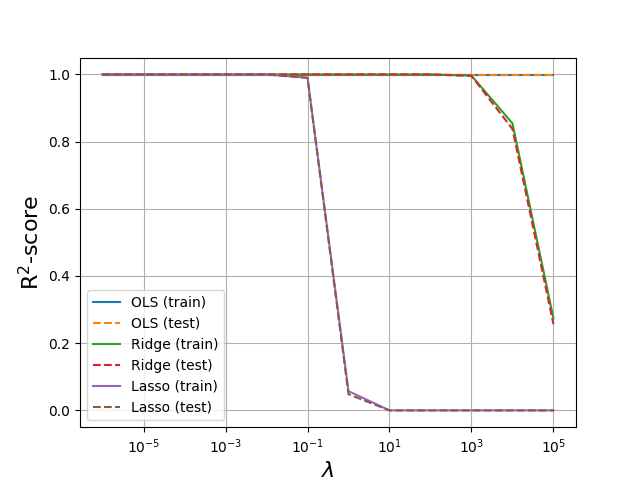
\includegraphics[scale=0.65]{../plots/lambda_vs_R2_linear.png}
	\caption{The R$^2$-score as a function of the penalty. }
	\label{fig:lambda_vs_R2_linear}
\end{figure} 
\fi

\begin{table} [H]
	\caption{The accuracy obtained using neural network for classification. 'Train' is the training set, 'Test' is a test set far from critical temperature and 'Critical' is a test set close to the critical temperature. We used one minimization iteration ($T=1$), learning rate $\eta=1e-4$ and regularization parameter $\lambda=1e-3$, used logistic activation function on output node and tried \textit{pure linear}, \textit{ReLU} and \textit{Leaky ReLU} on the hidden layers. Notation "10+10" means two layers of 10 hidden nodes each.}
	\begin{tabularx}{\textwidth}{l|l|XXX} \hline\hline
		\label{tab:nn_class}
		&& \multicolumn{3}{c}{\textbf{Accuracy}}\\ \hline
		&Hidden nodes&Train&Test&Critical\\ \hline
		
		\parbox[t]{2mm}{\multirow{3}{*}{\rotatebox[origin=c]{90}{Linear}}}
		&10 & 0.4371 & 0.4381 & 0.3333 \\
		&10+10 & 0.4379 & 0.4367 & 0.3333 \\
		&10+10+10 & 0.4371 & 0.4382 & 0.3333 \\ \hline
		
		\parbox[t]{2mm}{\multirow{3}{*}{\rotatebox[origin=c]{90}{ReLU}}}
		&10 & 0.9930 & 0.9929 & 0.9655 \\
		&10+10 & 0.9935 & 0.9934 & 0.9679 \\
		&10+10+10 & 0.9935 & \textbf{0.9938} & \textbf{0.9686} \\ \hline
		
		\parbox[t]{2mm}{\multirow{3}{*}{\rotatebox[origin=c]{90}{Leaky}}}
		&10 & 0.9931 & 0.9929 & 0.9656 \\
		&10+10 & 0.9932 & 0.9933 & 0.9668 \\
		&10+10+10 & \textbf{0.9936} & 0.9935 & 0.9685 \\ \hline\hline
	\end{tabularx}
\end{table}

\subsection{Feed-forward Neural Networks}

\subsection{Convolutional Neural Networks}

\subsection{Recurrent Neural Networks}

